\documentclass[dvipdfmx]{jsarticle}


\usepackage{tcolorbox}
\usepackage{color}
\usepackage{listings, plistings}

%% ノート/latexメモ
%% http://pepper.is.sci.toho-u.ac.jp/pepper/index.php?%A5%CE%A1%BC%A5%C8%2Flatex%A5%E1%A5%E2

%% JavaScriptの設定
%% https://e8l.hatenablog.com/entry/2015/11/29/232800
\lstdefinelanguage{javascript}{
  morekeywords = [1]{ %keywords
    await, break, case, catch, class, const, continue, debugger, default, delete, 
    do, else, enum, export, extends, finally, for, function, function*, if, implements, import, in, 
    instanceof, interface, let, new, package, private, protected, public, return, static, super,
    switch, this, throw, try, typeof, var, void, while, with, yield, yield*
  },
  morekeywords = [2]{ %literal
    false, Infinity, NaN, null, true, undefined
  },
  morekeywords = [3] { %Classes
    Array, ArrayBuffer, Boolean, DataView, Date, Error, EvalError, Float32Array, Float64Array,
    Function, Generator, GeneratorFunction, Int16Array, Int32Array, Int8Array, InternalError,
    JSON, Map, Math, Number, Object, Promise, Proxy, RangeError, ReferenceError, Reflect,
    RegExp, Set, String, Symbol, SyntaxError, TypeError, URIError, Uint16Array, Uint32Array,
    Uint8Array, Uint8ClampedArray, WeakMap, WeakSet
  },
  morecomment = [l]{//},
  morecomment = [s]{/*}{*/},
  morestring = [b]{"},
  morestring = [b]{'},
  alsodigit = {-},
  sensitive = true
}

%% 修正時刻: Tue 2022/03/15 10:04:41


% Java
\lstset{% 
  frame=single,
  backgroundcolor={\color[gray]{.9}},
  stringstyle={\ttfamily \color[rgb]{0,0,1}},
  commentstyle={\itshape \color[cmyk]{1,0,1,0}},
  identifierstyle={\ttfamily}, 
  keywordstyle={\ttfamily \color[cmyk]{0,1,0,0}},
  basicstyle={\ttfamily},
  breaklines=true,
  xleftmargin=0zw,
  xrightmargin=0zw,
  framerule=.2pt,
  columns=[l]{fullflexible},
  numbers=left,
  stepnumber=1,
  numberstyle={\scriptsize},
  numbersep=1em,
  language={Java},
  lineskip=-0.5zw,
  morecomment={[s][{\color[cmyk]{1,0,0,0}}]{/**}{*/}},
  keepspaces=true,         % 空白の連続をそのままで
  showstringspaces=false,  % 空白字をOFF
}
%\usepackage[dvipdfmx]{graphicx}
\usepackage{url}
\usepackage[dvipdfmx]{hyperref}
\usepackage{amsmath, amssymb}
\usepackage{itembkbx}
\usepackage{eclbkbox}	% required for `\breakbox' (yatex added)
\usepackage{enumerate}
\usepackage[default]{cantarell}
\usepackage[T1]{fontenc}
\fboxrule=0.5pt
\parindent=1em
\definecolor{mygrey}{rgb}{0.97, 0.97, 0.97}

\makeatletter
\def\verbatim@font{\normalfont
\let\do\do@noligs
\verbatim@nolig@list}
\makeatother

\begin{document}

%\anaumeと入力すると穴埋め解答欄が作れるようにしてる。\anaumesmallで小さめの穴埋めになる。
\newcounter{mycounter} % カウンターを作る
\setcounter{mycounter}{0} % カウンターを初期化
\newcommand{\anaume}[1][]{\refstepcounter{mycounter}{#1}{\boxed{\phantom{aa}\textnormal{\themycounter}\phantom{aa}}}} %穴埋め問題の空欄作ってる。
\newcommand{\anaumesmall}[1][]{\refstepcounter{mycounter}{#1}{\boxed{\tiny{\phantom{a}\themycounter \phantom{a}}}}}%小さい版作ってる。色々改造できる。

%% 修正時刻: Tue 2022/03/15 10:04:411


\section{ちょっと複雑なデータベースを考える}

\subsection{データベースの例}

今度は以下のようなデータについて考えてみる。

\vspace{3mm}
 \begin{tabular}{|l|l|} \hline
  氏名 & 菅原文太 \\
  性別 & 男性 \\
  年齢 & 40歳 \\
  誕生年 & 1933年生まれ \\
  部署 & 総務部 \\ 
  趣味 & 釣り、油絵、空手  \\ \hline
 \end{tabular}

\vspace{3mm}
 \begin{tabular}{|l|l|} \hline
  氏名 & 千葉真一 \\
  性別 & 男性 \\
  年齢 & 34歳 \\
  誕生年 &  1939年生まれ \\
  部署 & 営業部 \\
  趣味 & 空手、熱帯魚飼育、サッカー観戦、釣り  \\ \hline
 \end{tabular}

\vspace{3mm}
 \begin{tabular}{|l|l|} \hline
  氏名 & 北大路欣也 \\
  性別 & 男性 \\
  年齢 & 30歳 \\
  誕生年 &  1943年生まれ \\
  部署 & 経理部 \\
  趣味 & 茶道、空手  \\ \hline
 \end{tabular}

\vspace{3mm}
 \begin{tabular}{|l|l|} \hline
  氏名 & 梶芽衣子 \\
  性別 & 女性 \\
  年齢 & 26歳 \\
  誕生年 &  1947年生まれ \\
  部署 & 営業部 \\
  趣味 & 登山、ヨガ、サッカー観戦  \\ \hline
 \end{tabular}
\vspace{3mm}

まず、このような表がイメージされる。

 emp表 \\
  \begin{tabular}[h]{|c|l|c|c|c|c|l|}
   \hline
   ID & 名前       & 性別 & 年齢 & 誕生年 & 部署 & 趣味 \\ \hline\hline
   1  & 菅原文太   & 男性 & 40   & 1933   & 総務 & 釣り, 油絵, 空手  \\ \hline
   2  & 千葉真一   & 男性 & 34   & 1939   & 営業 & 空手, 熱帯魚飼育, サッカー観戦, 釣り \\ \hline
   3  & 北大路欣也 & 男性 & 30   & 1943   & 経理 & 茶道, 空手 \\ \hline
   4  & 梶芽衣子   & 女性 & 26   & 1947   & 営業 & 登山, ヨガ, サッカー観戦  \\ \hline
  \end{tabular}

しかしながら、この表の場合、趣味のフィールドには、複数のデータが含まれている。
これを解消したのが、次の表である。


\subsection{第1正規形}

\vspace{3mm}
emp表 \\
  \begin{tabular}[h]{|c|l|c|c|c|c|l|l|l|l|}
   \hline
   \underline{ID}
      & 名前       & 性別 & 年齢 & 誕生年 & 部署 & 趣味1 & 趣味2     & 趣味3       & 趣味4 \\ \hline\hline
   1  & 菅原文太   & 男性 & 40   & 1933   & 総務 & 釣り & 油絵       & 空手        &      \\ \hline
   2  & 千葉真一   & 男性 & 34   & 1939   & 営業 & 空手 & 熱帯魚飼育 & サッカー観戦 & 釣り \\ \hline
   3  & 北大路欣也 & 男性 & 30   & 1943   & 経理 & 茶道 & 空手       &             & \\ \hline
   4  & 梶芽衣子   & 女性 & 26   & 1947   & 営業 & 登山 & ヨガ       & サッカー観戦 & \\ \hline
  \end{tabular}
\vspace{3mm}


趣味のフィールドが1つのもの、3つのものとバラバラなので、フィールドを1つにする。

\vspace{3mm}
  emp表 \\
  \begin{tabular}[h]{|c|l|c|c|c|c|l|}
   \hline
   \underline{ID}
      & 名前        & 性別 & 年齢 & 誕生年 & 部署 & 趣味 \\ \hline\hline
   1  & 菅原文太    & 男性 & 40   & 1933   & 総務 & 釣り \\ \hline
   1  & 菅原文太    & 男性 & 40   & 1933   & 総務 & 油絵 \\ \hline
   1  & 菅原文太    & 男性 & 40   & 1933   & 総務 & 空手 \\ \hline
   2  & 千葉真一    & 男性 & 34   & 1939   & 営業 & 空手  \\ \hline
   2  & 千葉真一    & 男性 & 34   & 1939   & 営業 & 熱帯魚飼育 \\ \hline
   2  & 千葉真一    & 男性 & 34   & 1939   & 営業 & サッカー観戦 \\ \hline
   2  & 千葉真一    & 男性 & 34   & 1939   & 営業 & 釣り \\ \hline
   3  & 北大路欣也  & 男性 & 30   & 1943   & 経理 & 茶道 \\ \hline
   3  & 北大路欣也  & 男性 & 30   & 1943   & 経理 & 空手 \\ \hline
   4  & 梶芽衣子    & 女性 & 26   & 1947   & 営業 & 登山 \\ \hline
   4  & 梶芽衣子    & 女性 & 26   & 1947   & 営業 & ヨガ \\ \hline
   4  & 梶芽衣子    & 女性 & 26   & 1947   & 営業 & サッカー観戦 \\ \hline
  \end{tabular}
\vspace{3mm}

ここまでが「第1正規化」で、この表を「第1正規形」と呼ぶ。

\vspace{5mm}
\begin{tcolorbox}
{\large \textgt{第1正規形} :\quad 1つのセルには1つの値しか含まない}
\end{tcolorbox}

\newpage
\subsection{第2正規形}


上の表は縦方向にデータが繰り返されている。
これを表を分けることによって、解消する。
名前、性別等の列は、主キーである \textsf{ID} に従属している。
趣味の列は、この表には隠れている別の主キー に従属していると考える。
今回の場合は、emp表の \textsf{ID} と hobby表の \textsf{HID} である。
この2つのキーを主キー(複合キー)として、それに従属していると考える。

\begin{multicols}{2}

 emp表 \\
  \begin{tabular}[h]{|c|l|c|c|c|c|}
   \hline
   \underline{ID}
      & 名前       & 性別 & 年齢 & 誕生年 & 部署  \\ \hline\hline
   1  & 菅原文太   & 男性 & 40   & 1933   & 総務  \\ \hline
   2  & 千葉真一   & 男性 & 34   & 1939   & 営業  \\ \hline
   3  & 北大路欣也 & 男性 & 30   & 1943   & 経理  \\ \hline
   4  & 梶芽衣子   & 女性 & 26   & 1947   & 営業  \\ \hline
  \end{tabular}

 \columnbreak

 hobby表 \\
  \begin{tabular}[h]{|c|l|}
   \hline
   \underline{HID}
         & 趣味 \\ \hline\hline
   H01   & 釣り \\ \hline
   H02   & 油絵 \\ \hline
   H03   & 空手  \\ \hline
   H04   & 熱帯魚飼育 \\ \hline
   H05   & サッカー観戦 \\ \hline
   H06   & 茶道 \\ \hline
   H07   & 登山 \\ \hline
   H08   & ヨガ \\ \hline
  \end{tabular}
\end{multicols}

\noindent
emp\_hobby表\\
\begin{tabular}{|c|c|cc} \cline{1-2}
 \multicolumn{2}{|c|}{主キー} & \multirow{2}{*}{名前} & \multirow{2}{*}{趣味} \\ \cline{1-2}
 \underline{ID} & \underline{HID} &   &   \\ \cline{1-2}\cline{1-2}
 1  & H01 & 菅原文太 &  釣り \\ \cline{1-2}
 1  & H02 & 菅原文太 & 油絵 \\ \cline{1-2}
 1  & H03 & 菅原文太 & 空手 \\ \cline{1-2}
 2  & H03 & 千葉真一 & 空手 \\ \cline{1-2}
 2  & H04 & 千葉真一 & 熱帯魚飼育 \\ \cline{1-2}
 2  & H05 & 千葉真一 & サッカー観戦 \\ \cline{1-2}
 2  & H01 & 千葉真一 & 釣り \\ \cline{1-2}
 3  & H06 & 北大路欣也 & 茶道 \\ \cline{1-2}
 3  & H03 & 北大路欣也 & 空手 \\ \cline{1-2}
 4  & H07 & 梶芽衣子 & 登山 \\ \cline{1-2}
 4  & H08 & 梶芽衣子 & ヨガ \\ \cline{1-2}
 4  & H05 & 梶芽衣子 & サッカー観戦 \\ \cline{1-2}
\end{tabular}

\vspace{3mm}
名前と趣味の列は、わかりやすくするためにつけた。
emp\_hobby表は、ID と HID の2つの列だけの表である。


\vspace{5mm}
\begin{tcolorbox}
{\large \textgt{第2正規形} :\quad 表の中に主キーが1つである。複合列が主キーとなっている場合は、主キーの1つだけに従属する列があってはならない。}
\end{tcolorbox}



\newpage
\subsection{第3正規形}

emp表には、表には現れていないが、id に従属せず、別のキーに従属すると
考えられるフィールドが存在する。それは「性別」と「所属」である。
これを別の表(gender表、dept表)とする。

\begin{multicols}{2}
 emp表 \\
  \begin{tabular}[h]{|c|l|c|c|}
   \hline
   \underline{ID}
      & 名前       & 年齢 & 誕生年 \\ \hline\hline
   1  & 菅原文太   & 40   & 1933   \\ \hline
   2  & 千葉真一   & 34   & 1939   \\ \hline
   3  & 北大路欣也 & 30   & 1943   \\ \hline
   4  & 梶芽衣子   & 26   & 1947   \\ \hline
  \end{tabular}

 \columnbreak

 gender表 \\
 \begin{tabular}{|c|c|} \hline
  \underline{GID}
      & 性別 \\  \hline\hline
  0   & 不明 \\ \hline
  1   & 男性 \\ \hline
  2   & 女性 \\ \hline
  3   & その他 \\ \hline
 \end{tabular}
\end{multicols}

\begin{multicols}{3}
 dept表 \\
 \begin{tabular}{|c|c|} \hline
  \underline{DID}
      & 部署名 \\ \hline\hline
  D01 & 総務部 \\ \hline
  D02 & 営業部 \\ \hline
  D03 & 経理部 \\ \hline
  D04 & 開発部 \\ \hline
 \end{tabular}
  
 \columnbreak

 hobby表 \\
  \begin{tabular}[h]{|c|l|}
   \hline
   \underline{HID}
         & 趣味 \\ \hline\hline
   H01   & 釣り \\ \hline
   H02   & 油絵 \\ \hline
   H03   & 空手  \\ \hline
   H04   & 熱帯魚飼育 \\ \hline
   H05   & サッカー観戦 \\ \hline
   H06   & 茶道 \\ \hline
   H07   & 登山 \\ \hline
   H08   & ヨガ \\ \hline
  \end{tabular}

 \columnbreak

 \noindent
 emp\_hobby表\\
 \begin{tabular}{|c|c|} \hline
  \multicolumn{2}{|c|}{主キー} \\ \hline
  \underline{ID} & \underline{HID}  \\ \hline\hline
  1  & H01  \\ \hline
  1  & H02  \\ \hline
  1  & H03  \\ \hline
  2  & H03  \\ \hline
  2  & H04  \\ \hline
  2  & H05  \\ \hline
  2  & H01  \\ \hline
  3  & H06  \\ \hline
  3  & H03  \\ \hline
  4  & H07  \\ \hline
  4  & H08  \\ \hline
  4  & H05  \\ \hline
 \end{tabular}
\end{multicols}

\vspace{5mm}
\begin{tcolorbox}
\large{\textgt{第3正規形} :\quad すべての列が主キーに従属している。}
\end{tcolorbox}


\newpage
\section{ER図}

第3正規形ができたところで、ER図を作ってみる。

\vspace{3mm}
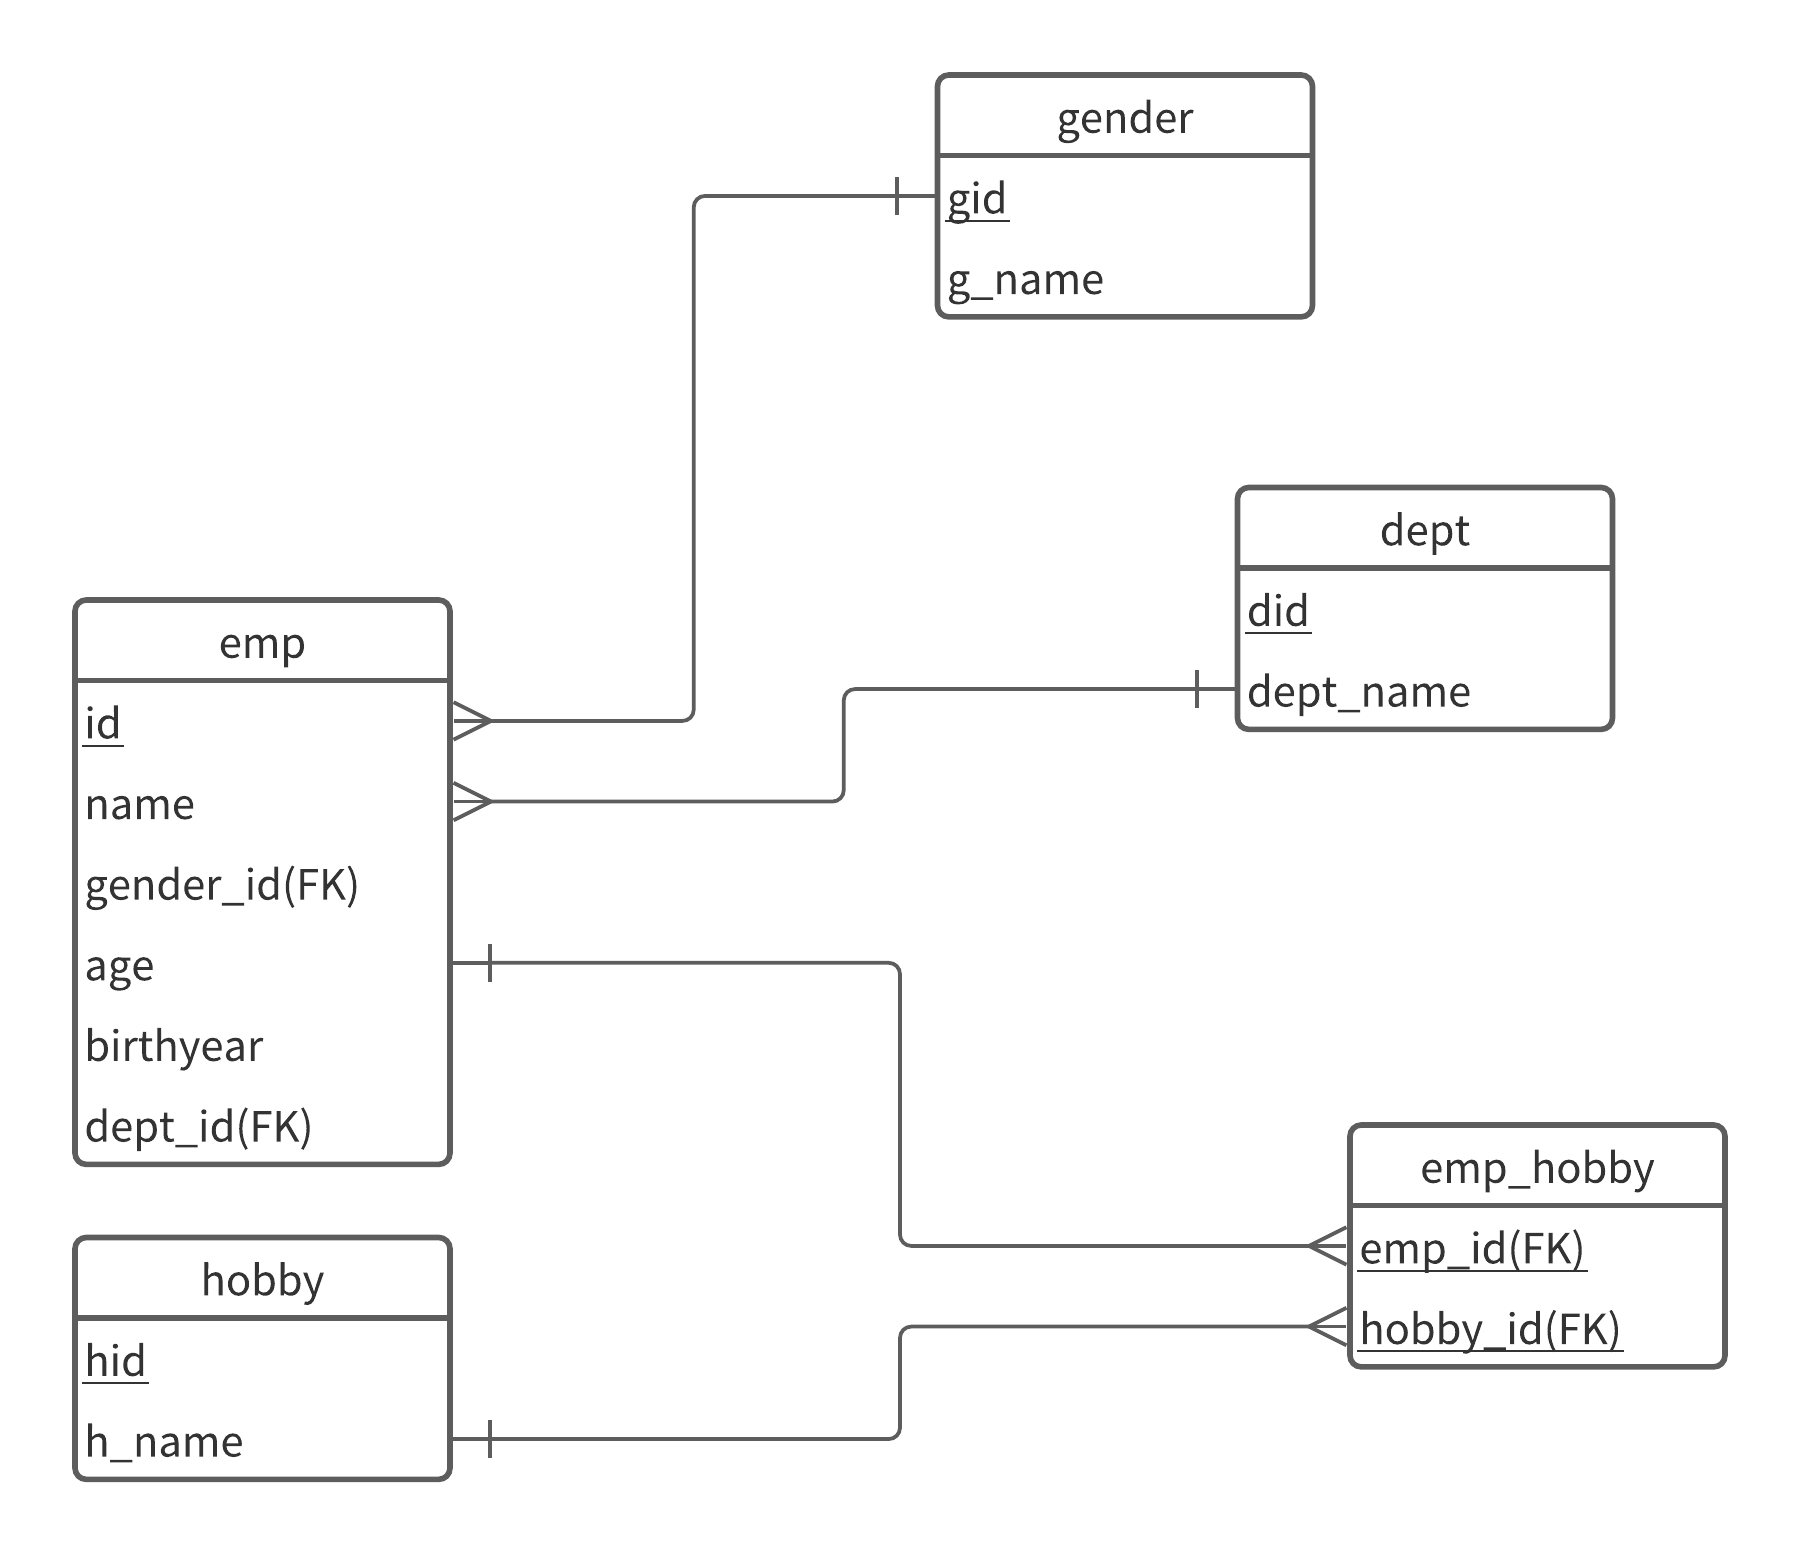
\includegraphics[width=14cm]{img/ER.png}
\vspace{3mm}

\vspace{3mm}
\begin{center}
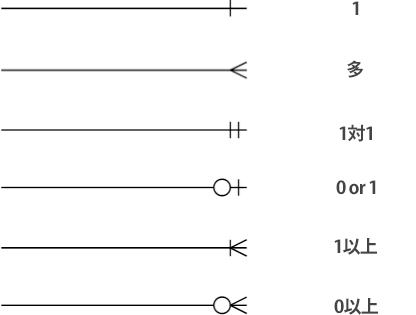
\includegraphics[width=6cm]{img/ERD-Notation-ja.png}
\end{center}
\vspace{3mm}


\newpage
\section{実際にデータベースを作ってみる}

\subsection{rootでMySQLサーバーにログインする}

以下のようなデータベースであるとする。

\begin{tcolorbox}
 データベース名 : \quad sample
\end{tcolorbox}

管理者(root) で MySQLサーバーにログインする。

\begin{lstlisting}[numbers=none, language=sql]
 > mysql -u root -p
 Password: ********
\end{lstlisting}

ます、データベースを作成する。
そして、sampleデータベースの使用を宣言する。

\begin{lstlisting}[language=SQL, numbers=none]
 MariaDB[(none)]> CREATE DATABASE sample;
 MariaDB[(none)]> USE sample;
\end{lstlisting}


\subsection{テーブルの定義}

以下のようにテーブルを定義する。

\begin{lstlisting}[caption=gender表, language=sql]
 MariaDB> CREATE TABLE gender (
     ->   gid CHAR(1) PRIMARY KEY,
     ->   gname VARCHAR(3) NOT NULL
     -> );
\end{lstlisting}

\begin{lstlisting}[caption=dept表, language=sql]
 MariaDB> CREATE TABLE dept (
     ->   did CHAR(3) PRIMARY KEY,
     ->   dname VARCHAR(20) NOT NULL
     -> );
\end{lstlisting}

\begin{lstlisting}[caption=emp表, language=sql]
 MariaDB> CREATE TABLE emp (
     ->   id INT AUTO_INCREMENT,
     ->   name VARCHAR(100) NOT NULL,
     ->   gender_id CHAR(1) NOT NULL,
     ->   age INT NOT NULL,
     ->   birthyear INT NOT NULL,
     ->   dept_id CHAR(3),
     ->   PRIMARY KEY (id)
     -> );
\end{lstlisting}

gender\_id に外部キー制約を追加する。参照先は gender表のgidである。

\begin{lstlisting}[caption=emp表, language=sql]
 MariaDB> ALTER TABLE emp
     -> ADD
     ->   CONSTRAINT fk_gender_id
     ->     FOREIGN KEY (gender_id)
     ->     REFERENCES gender (gid);
\end{lstlisting}

dept\_id に外部キー制約を追加する。参照先は dept表のdidである。

\begin{lstlisting}[caption=emp表, language=sql]
 MariaDB> ALTER TABLE emp
     -> ADD
     ->   CONSTRAINT fk_dept_id
     ->     FOREIGN KEY (dept_id)
     ->     REFERENCES dept (did);
\end{lstlisting}

hobby表を定義する。

\begin{lstlisting}[caption=hobby表, language=sql]
 mysql> CREATE TABLE hobby (
     ->   hid CHAR(3) PRIMARY KEY,
     ->   hname VARCHAR(20) NOT NULL
     -> );
\end{lstlisting}

誰がどういう趣味を持っているかの対応表を作成する。
この表では、カラムid と カラムhid の2つセットで主キーとなる。
(複合主キー)

\begin{lstlisting}[caption=emp\_hobby表, language=sql]
 mysql> CREATE TABLE emp_hobby (
     ->   id INT NOT NULL,
     ->   hid CHAR(3) NOT NULL,
     ->   PRIMARY KEY (id, hid)
     -> );
\end{lstlisting}

\subsection{データの登録}

gender表のデータは全部で4件である。gidはchar型1文字である。

\begin{lstlisting}[caption=gender表]
INSERT INTO gender
  (gid, gname)
VALUES
  ('0', '不明'),
  ('1', '男性'),
  ('2', '女性'),
  ('3', 'その他');
\end{lstlisting}

dept表のデータを入力する。didはchar型3文字である。

\begin{lstlisting}[caption=dept表]
INSERT INTO dept
  (did, dname)
VALUES
  ('001', '総務部'),
  ('002', '営業部'),
  ('003', '経理部'),
  ('004', '開発部'); 
\end{lstlisting}

emp表を入力する。idは自動連番である。

\begin{lstlisting}[caption=emp表]
INSERT INTO emp
  (name, gender_id, age, birthyear, dept_id)
VALUES
  ('菅原文太', '1', 40, 1933, '001'),
  ('千葉真一', '1', 34, 1939, '002'),
  ('北大路欣也', '1', 30, 1943, '003'),
  ('梶芽衣子', '2', 26, 1947, '002'); 
\end{lstlisting}

hobby表を入力する。

\begin{lstlisting}[caption=hobby]
INSERT INTO hobby
  (hid, hname)
VALUES
  ('H01', '釣り'),
  ('H02', '油絵'),
  ('H03', '空手'),
  ('H04', '熱帯魚飼育'),
  ('H05', 'サッカー観戦'),
  ('H06', '茶道'),
  ('H07', '登山'),
  ('H08', 'ヨガ'); 
\end{lstlisting}

社員と趣味との対応表の入力である。

\begin{lstlisting}[caption=emp\_hobby]
INSERT INTO emp_hobby
  (id, hid)
VALUES
  (1, 'H01'),
  (1, 'H02'),
  (1, 'H03'),
  (2, 'H03'),
  (2, 'H04'),
  (2, 'H05'),
  (2, 'H01'),
  (3, 'H06'),
  (3, 'H03'),
  (4, 'H07'),
  (4, 'H08'),
  (4, 'H05'); 
\end{lstlisting}

\subsection{データを表示する}

以下のように4つの表を結合する。

\begin{lstlisting}[language=sql, numbers=none]
 MariaDB> SELECT
   ->   e.name AS 名前,
   ->   g.gname AS 性別,
   ->   d.dname AS 所属,
   ->   h.hname AS 趣味
   -> FROM emp e
   -> INNER JOIN emp_hobby eh
   -> ON eh.id = e.id
   ->   INNER JOIN gender g
   ->   ON g.gid = e.gender_id
   ->     INNER JOIN dept d
   ->     ON d.did = e.dept_id
   ->       INNER JOIN hobby h
   ->       ON h.hid = eh.hid
   -> ORDER BY e.id;
\end{lstlisting}

結合表を表示するたびに、この長いコマンドを入力するのは大変なので、
(エディタに記述しておいて、必要なときにコピー貼り付けしてもいいのだが)
ビューという形でデータベース内にこのコマンドを登録しておくことができる。

以下のように ビュー を作成してみた。

\begin{lstlisting}[language=sql, numbers=none]
MariaDB> CREATE VIEW hobby_view AS
   -> SELECT
   ->   e.name AS 名前,
   ->   g.gname AS 性別,
   ->   d.dname AS 所属,
   ->   h.hname AS 趣味
   -> FROM emp e
   -> INNER JOIN emp_hobby eh
   -> ON eh.id = e.id
   ->   INNER JOIN gender g
   ->   ON g.gid = e.gender_id
   ->     INNER JOIN dept d
   ->     ON d.did = e.dept_id
   ->       INNER JOIN hobby h
   ->       ON h.hid = eh.hid 
   -> ORDER BY e.id;
\end{lstlisting}

こうしておくと、

\begin{lstlisting}[language=sql, numbers=none]
 MariaDB> SELECT * FROM hobby_view;
\end{lstlisting}

とするだけで、先の結合表を表示できる。
また、次のように、検索・表示もできる。

\begin{lstlisting}[language=sql, numbers=none]
 MariaDB> SELECT * FROM hobby_view
    -> WHERE 趣味 LIKE '%空手%';
\end{lstlisting}


\begin{lstlisting}[caption=出力例, numbers=none]
+-----------------+--------+-----------+--------+
| 名前            | 性別    | 所属      | 趣味    |
+-----------------+--------+-----------+--------+
| 菅原文太         | 男性    | 総務部    | 空手    |
| 千葉真一         | 男性    | 営業部    | 空手    |
| 北大路欣也       | 男性    | 経理部    | 空手    |
+-----------------+--------+-----------+--------+
\end{lstlisting}


\end{document}

%% 修正時刻: Sat May  2 15:10:04 2020


%% 修正時刻: Tue 2023/10/03 06:54:002
